
\subsection{定理 Y 的证明}
\label{subsec:7-4-6}
\liftIndex{I180}

考虑定理~\ref{thm:4-6-52} 的情形。
也就是说，假设存在辛微分同胚
\[
\psi\colon M\longrightarrow M'
\]
使得 $\psi(L)=L'$。
由定理~\ref{thm:4-6-1} 与
定理~\ref{thm:7-4-41}，
存在滤过 $L_\infty$ 同伦等价
\begin{equation}
\psi_*\colon
\operatorname{Der}B
\bigl(H(L;\Lambda_{0,\mathrm{nov}})[1]\bigr)
\longrightarrow
\operatorname{Der}B
\bigl(H(L';\Lambda_{0,\mathrm{nov}})[1]\bigr).
\tag{7.4.119}\label{eq:7-4-119}
\end{equation}
把系数环约化为 $\mathbb Q$ 后，
同态~\eqref{eq:7-4-119}
诱导线性同构
\[
H(L;\mathbb Q)\cong H(L';\mathbb Q).
\]

\begin{theorem}{7.4.120}\label{thm:7-4-120}
可以选取 $\psi_*$，
使下列图式在严格滤过 $L_\infty$ 同伦意义下交换。

\par\medskip\noindent\begin{minipage}{\textwidth}
\centering
\resizebox{.9\textwidth}{!}{$\displaystyle
\begin{array}{ccc}
H(M;\Lambda_{0,\mathrm{nov}})[1]
&\xrightarrow{\ \mathfrak q^\circ\ }&
\operatorname{Der}B\bigl(H(L;\Lambda_{0,\mathrm{nov}})[1]\bigr)
\\[-0.1em]
{\scriptstyle\psi_*}\Big\downarrow
&&
\Big\downarrow{\scriptstyle\psi_*}
\\[-0.1em]
H(M';\Lambda_{0,\mathrm{nov}})[1]
&\xrightarrow{\ \mathfrak q^\circ\ }&
\operatorname{Der}B\bigl(H(L';\Lambda_{0,\mathrm{nov}})[1]\bigr)
\end{array}$}
\par\smallskip
{\renewcommand{\thefigure}{7.4.1}\refstepcounter{figure}
\normalfont\bfseries 图式~\thefigure\label{diag:7-4-1}}
\end{minipage}\par\medskip
\end{theorem}

定理~\ref{thm:7-4-118}、
定理~\ref{thm:7-4-120}
再连同含幺版本，将蕴含定理~\ref{thm:intro-Y}。

\begin{proof}
与前面一样，只须证明 $A_{n,K}$ 版本。
考虑下列图式：

\par\medskip\noindent\begin{minipage}{\textwidth}
\centering
\resizebox{\textwidth}{!}{$\displaystyle
\begin{array}{ccccc}
C(L,\lambda)
&\xleftarrow{\ \operatorname{Eval}_{\rho=0}\ }&
C([0,1]\times L';\lambda,\lambda')
&\xrightarrow{\ \operatorname{Eval}_{\rho=1}\ }&
C(L';\lambda')
\\[-0.1em]
\Big\uparrow&&\Big\uparrow&&\Big\uparrow
\\[-0.1em]
H^*(L;\Lambda_{0,\mathrm{nov}})
&\xleftarrow{\ \operatorname{Eval}_{\rho=0}\ }&
H^*([0,1]\times L';\Lambda_{0,\mathrm{nov}})
&\xrightarrow{\ \operatorname{Eval}_{\rho=1}\ }&
H^*(L';\Lambda_{0,\mathrm{nov}})
\end{array}$}
\par\smallskip
{\renewcommand{\thefigure}{7.4.2}\refstepcounter{figure}
\normalfont\bfseries 图式~\thefigure\label{diag:7-4-2}}
\end{minipage}\par\medskip

该图式由图式~\ref{diag:7-2-37}
及定理~\ref{thm:5-4-2} 得到。
（图式~\ref{diag:7-4-2} 的交换性
见下文引理~\ref{lem:7-4-121} 的证明。）
图式右上角依既定记号写成
$C(L';\lambda')$\translatornote{源图写作 $C(L':\lambda')$，误以冒号分隔底空间与阶参数；译稿依同图其余对象及图式 7.2.35 改用分号。见疑误 A-0585。}。

证明的主要部分，是构造下列交换图式；
图中省略系数环 $\Lambda_{0,\mathrm{nov}}$。

\par\medskip\noindent\begin{minipage}{\textwidth}
\centering
\resizebox{\textwidth}{!}{$\displaystyle
\begin{array}{ccccc}
H(M)[1]
&\xrightarrow{\ \psi_*\ }&
H(M')[1]
&=&
H(M')[1]
\\[-0.1em]
{\scriptstyle\widehat{\mathfrak q}^{\circ}}\Big\downarrow
&&
{\scriptstyle\widehat{\mathfrak q}^{\circ}_{\mathrm{fami}}}\Big\downarrow
&&
{\scriptstyle\widehat{\mathfrak q}^{\circ}}\Big\downarrow
\\[-0.1em]
\operatorname{Der}B(C(L,\lambda)[1])
&&
\operatorname{Der}B(C([0,1]\times L';\lambda,\lambda')[1])
&&
\operatorname{Der}B(C(L';\lambda')[1])
\\[-0.1em]
\Big\downarrow&&\Big\downarrow&&\Big\downarrow
\\[-0.1em]
\operatorname{Der}B(H^*(L)[1])
&\xleftarrow{\ \operatorname{Eval}_{\rho=0}\ }&
\operatorname{Der}B(H^*([0,1]\times L')[1])
&\xrightarrow{\ \operatorname{Eval}_{\rho=1}\ }&
\operatorname{Der}B(H^*(L')[1])
\end{array}$}
\par\smallskip
{\renewcommand{\thefigure}{7.4.3}\refstepcounter{figure}
\normalfont\bfseries 图式~\thefigure\label{diag:7-4-3}}
\end{minipage}\par\medskip

由于图式~\ref{diag:7-4-2} 第二行中的箭头
都是同构，便得到图式~\ref{diag:7-4-3}
第三行中的箭头。
图式~\ref{diag:7-4-3} 下半部从
$\operatorname{Der}B(C(L,\lambda)[1])$ 等对象
到 $\operatorname{Der}B(H^*(L)[1])$ 等对象的
三根竖箭头，已在定理~\ref{thm:7-4-41}
的证明中构造。

\begin{lemma}{7.4.121}\label{lem:7-4-121}
存在 $\widehat{\mathfrak q}^{\circ}_{\mathrm{fami}}$，
使图式~\ref{diag:7-4-3} 交换。
\end{lemma}

\begin{proof}
考虑第~3.8.6 小节构造 $\mathfrak q$ 时所用的模空间
\[
\mathcal M_{k+1,\ell}(J,L';\beta).
\]
这里在记号中明确写出殆复结构 $J$，
因为下文将让它变化。
考虑第~\ref{subsec:7-2-14} 小节构造
图式~\ref{diag:7-2-35} 时所用的
$M'$ 上殆复结构族 $\{J_\rho\}_\rho$。
置
\begin{equation}
\begin{aligned}
&\mathcal M_{k+1,\ell}
(\{J_\rho\}_\rho,L';\beta;
\operatorname{twp}(\rho))\\
&\qquad=
\bigcup_{\rho\in[0,1]}
\{\rho\}\times
\mathcal M_{k+1,\ell}(J_\rho,L';\beta).
\end{aligned}
\tag{7.4.122}\label{eq:7-4-122}
\end{equation}
然后用它实行 $\mathfrak q$ 构造的单参数族版本，
得到
$\mathfrak q_{\mathrm{fami};\ell,k,\beta}$、
$\widehat{\mathfrak q}^{\circ}_{\mathrm{fami}}$ 等。

下面证明图式~\ref{diag:7-4-3} 的交换性。
先注意，可以选取模空间~\eqref{eq:7-4-122}
与 $\vec Q,\vec P$ 的纤维积之扰动，
使之与定义 $\mathfrak q_{\ell,k,\beta}$ 时所用的
\[
\mathcal M_{k+1,\ell}(L,\beta)
\mathbin{\times_{M^\ell\times L^k}}
\bigl(\vec Q\times
\operatorname{Eval}_{\rho=0}\vec P\bigr)
\]
的一个扰动相容。
于是有等式
\begin{equation}
\begin{aligned}
&\operatorname{Eval}_{\rho=0}\Bigl(
\mathfrak q_{\mathrm{fami};\ell,k,\beta}
(\psi_*\vec Q)(\vec P)\Bigr)\\
&\qquad=
\mathfrak q_{\ell,k,\beta}(\vec Q)
\bigl(\operatorname{Eval}_{\rho=0}\vec P\bigr).
\end{aligned}
\tag{7.4.123}\label{eq:7-4-123}
\end{equation}

我们在上链复形 $C(L;\lambda)$ 中选取
上同调类代表，使图式~\ref{diag:7-4-2} 交换；
并且选取格林算子 $\mathfrak G$，
使其与 $\operatorname{Eval}_{\rho=0}$ 交换。
利用式~\eqref{eq:7-4-123} 及这些事实，
即可证明图式~\ref{diag:7-4-3} 左半部交换。
（只须查看定理~\ref{thm:7-4-41}
证明中的运算定义。）
右半部的交换性以同样方式证明。
\end{proof}

由图式~\ref{diag:7-4-3} 的交换性，
定理~\ref{thm:7-4-120} 立即得证
\translatornote{源书此处误写“定理 7.4.118 得证”；当前证明自始至终针对定理 7.4.120，而 7.4.118 已在本小节之前证明。见疑误 A-0586。}。
\end{proof}

\begin{remark}{7.4.124}\label{rem:7-4-124}
\par\noindent\textup{(1)}
可以用上面证明的定理~\ref{thm:7-4-120}
的 $A_{n,K}$ 版本代替命题~\ref{prop:4-6-55}，
完成构造 $\mathfrak q$ 的最后一步，
即从 $A_{n,K}$ 版本过渡到 $A_\infty$ 版本。
另一方面，正如注~\ref{rem:7-2-303}(1) 所述，
在本书写作时，作者尚不知道如何以配边论证
（例如使用命题~\ref{prop:4-6-55}）
完成定理~\ref{thm:7-4-120} 的证明细节。

\par\noindent\textup{(2)}
对于构造中各种选择而言，
应当如何最恰当地陈述 $\psi_*$ 的同伦类
与这些选择无关，作者尚不清楚
\translatornote{源书这里及本项下文都只写 $\psi$；但给定的辛微分同胚 $\psi$ 不依赖这些辅助选择，定理 7.4.120 中实际由构造选取的是 $\psi_*$。见疑误 A-0587。}。
仔细考察定理~\ref{thm:7-4-41} 的证明可见，
并不容易说明同伦等价
\[
\operatorname{Der}B(\overline C[1])
\longrightarrow
\operatorname{Der}B(\overline H[1])
\]
究竟在何种意义下不依赖包含映射
$\overline H\to\overline C$
及格林算子 $\mathfrak G$ 的选取。
（当 $\overline C$ 是 de Rham 复形、
$\overline H$ 是 de Rham 上同调群时，
这些选择例如对应于黎曼度量的选取。）
不过，$\overline H$ 上的 $A_\infty$ 结构
在同构意义下不依赖这些选择。
定理~\ref{thm:7-4-120} 蕴含
$\psi_*$ 在相差
$\operatorname{Der}B(\overline H[1])$
自同构的意义下不依赖这些选择；
但作者不能确定这是否是最恰当的陈述。

使这种无关性难以透明呈现的一个原因是，
对应
\[
\overline C\longmapsto
\operatorname{Der}B(\overline C[1])
\]
既不协变，也不反变。

另一方面，$L_\infty$ 结构与高亏格版本
有更自然的联系，尤其与 $\overline C$ 的某种
Whitehead 扭率有关。
$\mathfrak G$ 的选取与使这种 Whitehead 扭率
良定义的选择有关。
若像第 4.6 节那样，
用滤过 $A_\infty$ 代数讨论良定义性，
这个问题便会消失。
通过 $L_\infty$ 结构研究良定义性，
在其高亏格推广的语境中似乎更自然。
本书把讨论限于亏格零情形，
故不再继续这一方向。
\end{remark}

下面说明定理~\ref{thm:intro-Y}
与第 3.8 节及第 4.6.4--4.6.6 小节讨论的关系
\liftIndex{I178}。
本小节余下论证可以显然地改写成含幺版本；
因此，下文省略含幺版本的讨论。

设 $C$ 为滤过 $A_\infty$ 代数，
并设
$\mathfrak B\in\operatorname{Der}B(C[1])$
为次数 $1$ 的元素。
考虑它的 Maurer--Cartan 方程
\begin{equation}
\delta(\mathfrak B)-[\mathfrak B,\mathfrak B]=0.
\tag{7.4.125}\label{eq:7-4-125}
\end{equation}
注意，由式~\eqref{eq:7-4-28} 定义的括号
$[\ ,\ ]$ 含有不寻常的因子 $-1/2$；
因此，式~\eqref{eq:7-4-125} 第二项的系数
与通常约定不同。
把
\[
\mathfrak B=(\mathfrak B_k)_{k\in\mathbb Z_{\ge0}},
\qquad
\mathfrak B_k\in
\operatorname{Hom}^{\mathrm{filt}}
\bigl(B_k(C[1]),C[1]\bigr)
\]
视为同一对象，并假设
\[
\mathfrak B_0\equiv0
\pmod{\Lambda^+_{0,\mathrm{nov}}}.
\]
置
\begin{equation}
\mathfrak m_k^{\mathfrak B}(x_1,\ldots,x_k)
=\mathfrak m_k(x_1,\ldots,x_k)
+\mathfrak B_k(x_1,\ldots,x_k).
\tag{7.4.126}\label{eq:7-4-126}
\end{equation}

\begin{lemma}{7.4.127}\label{lem:7-4-127}
$\mathfrak B$ 满足式~\eqref{eq:7-4-125}，
当且仅当 $\mathfrak m_k^{\mathfrak B}$
在 $C$ 上定义一个滤过 $A_\infty$ 代数结构。
\end{lemma}

\begin{proof}
由 $\mathfrak m_k^{\mathfrak B}$ 诱导的余导子
\[
\widehat d^{\mathfrak B}\colon
B(C[1])\longrightarrow B(C[1])
\]
等于 $\widehat d+\mathfrak B$，
其中 $\widehat d$ 由 $\mathfrak m_k$ 诱导。
因此
\[
\widehat d^{\mathfrak B}\circ
\widehat d^{\mathfrak B}
=\widehat d\circ\mathfrak B
+\mathfrak B\circ\widehat d
+\mathfrak B\circ\mathfrak B
=\delta(\mathfrak B)-[\mathfrak B,\mathfrak B].
\]
引理得证。
\end{proof}

\begin{remark}{7.4.128}\label{rem:7-4-128}
式~\eqref{eq:7-4-125} 可写成
\begin{equation}
\mathfrak l_1(\mathfrak B)
+\mathfrak l_2(\mathfrak B,\mathfrak B)=0,
\tag{7.4.125$'$}\label{eq:7-4-125-prime}
\end{equation}
这是 Maurer--Cartan 方程的 $L_\infty$ 版本
\begin{equation}
\widehat d(e^{\mathfrak B})=0
\tag{7.4.129}\label{eq:7-4-129}
\end{equation}
的一个特例\liftIndex{I068}\liftIndex{I078}。
（注意 $\deg\mathfrak B=1$。）
式~\eqref{eq:7-4-28} 前的负号
似乎正是使这里与 $L_\infty$ 表述相容所必需的。
\end{remark}

由于 $H^2(M;\Lambda_{0,\mathrm{nov}})$ 上的
Maurer--Cartan 方程是平凡的，
由定理~\ref{thm:intro-Y}，
每个 $b\in H^2(M;\Lambda_{0,\mathrm{nov}})$ 都诱导
\[
\mathfrak q^\circ_*(e^b)
=\mathfrak B
\in
\operatorname{Der}B
\bigl(C(L;\Lambda_{0,\mathrm{nov}})[1]\bigr),
\]
它满足式~\eqref{eq:7-4-125}，
因而由引理~\ref{lem:7-4-127}
把 $\mathfrak m$ 形变为 $\mathfrak m^{\mathfrak B}$。
这与定义~\ref{def:3-8-38} 中定义的
滤过 $A_\infty$ 结构
$\mathfrak m^b=\mathfrak m^{b,0}$ 一致
\liftIndex{I178}。

下面继续这一讨论，并证明定理~\ref{thm:4-6-47}。
对滤过 $L_\infty$ 代数 $\mathcal C$，
以 $\widehat{\mathcal M}(\mathcal C)$
表示式~\eqref{eq:7-4-129} 的所有解所成集合。

\begin{definition}{7.4.130}\label{def:7-4-130}
设
$\mathfrak B,\mathfrak B'
\in\widehat{\mathcal M}(\mathcal C)$。
若存在
\[
\widetilde{\mathfrak B}
\in
\widehat{\mathcal M}
\bigl(\operatorname{Poly}([0,1],\mathcal C)\bigr)
\]
使得
\begin{equation}
\operatorname{Eval}_{s=0}\widetilde{\mathfrak B}
=\mathfrak B,
\qquad
\operatorname{Eval}_{s=1}\widetilde{\mathfrak B}
=\mathfrak B',
\tag{7.4.131}\label{eq:7-4-131}
\end{equation}
则称 $\mathfrak B$ 与 $\mathfrak B'$ 规范等价，
并记作 $\mathfrak B\sim\mathfrak B'$。
\end{definition}

与 $A_\infty$ 情形相同，可以证明：
$\sim$ 是等价关系；
$\mathcal C\mapsto\mathcal M(\mathcal C)$
是同伦函子，其中
$\mathcal M(\mathcal C)$
是所有 $\sim$ 等价类所成集合。

现在考虑
$\mathcal C=\operatorname{Der}B(C[1])$ 的情形。
设
\[
\mathfrak B,\mathfrak B'
\in
\widehat{\mathcal M}
\bigl(\operatorname{Der}B(C[1])\bigr).
\]
假设 $C$ 有隙，且
\[
\mathfrak B
=\sum_{(\lambda_i,n_i)\in G}
\mathfrak B_iT^{\lambda_i}e^{n_i/2},
\qquad
\mathfrak B'
=\sum_{(\lambda_i,n_i)\in G}
\mathfrak B'_iT^{\lambda_i}e^{n_i/2}.
\]
若式~\eqref{eq:7-4-131} 中的
$\widetilde{\mathfrak B}$
还可取成这种形式，
就称 $\mathfrak B$ 与 $\mathfrak B'$
$G$-规范等价\liftIndex{I336}。

\begin{theorem}{7.4.132}\label{thm:7-4-132}
若 $\mathfrak B$ 与 $\mathfrak B'$
$G$-规范等价，
则 $(C,\mathfrak m^{\mathfrak B})$
与 $(C,\mathfrak m^{\mathfrak B'})$
严格、$G$-有隙且滤过地同伦等价。
\end{theorem}

\begin{proof}
首先定义
\begin{equation}
\Phi\colon
\operatorname{Poly}
\bigl([0,1],\operatorname{Der}B(C[1])\bigr)
\longrightarrow
\operatorname{Der}B
\bigl(\operatorname{Poly}([0,1],C[1])\bigr).
\tag{7.4.133}\label{eq:7-4-133}
\end{equation}
令
\[
\widetilde Y
=Y(s)+ds\wedge Z(s)
\in
\operatorname{Poly}
\bigl([0,1],\operatorname{Der}B(C[1])\bigr).
\]
（把第二项写成 $ds\wedge Z(s)$，
比写成 $Z(s)\wedge ds$ 更符合本书的符号约定。）
置
\[
\Phi(\widetilde Y)
(\mathbf x_1,\ldots,\mathbf x_k)
=\mathbf x,
\]
其中
\[
\mathbf x_i=x_i(s)+ds\wedge y_i(s),
\qquad
\mathbf x=x(s)+ds\wedge y(s),
\]
且
\[
x(s)=Y(s)
\bigl(x_1(s),\ldots,x_k(s)\bigr),
\]
\[
\begin{aligned}
y(s)={}&
\sum_i(-1)^{*_i}Y(s)
\bigl(x_1(s),\ldots,y_i(s),\ldots,x_k(s)\bigr)\\
&+Z(s)\bigl(x_1(s),\ldots,x_k(s)\bigr).
\end{aligned}
\]
这里
\[
*_i=\deg' x_1+\cdots+\deg' x_{i-1}+\deg Y.
\]
第 A4 节将核验，包括符号在内，
$\Phi$ 是微分分次李代数同态。

由引理~\ref{lem:7-4-127} 与式~\eqref{eq:7-4-133}，
得到滤过 $A_\infty$ 代数
\[
\Bigl(
\operatorname{Poly}([0,1],C),
\mathfrak m^{\Phi_*(\widetilde{\mathfrak B})}
\Bigr),
\]
其中 $\Phi_*$ 由引理~\ref{lem:3-6-36}
从 $\Phi$ 诱导。
按构造，有滤过 $A_\infty$ 同态
\[
\begin{aligned}
\operatorname{Eval}_{s=0}\colon
\Bigl(\operatorname{Poly}([0,1],C),
\mathfrak m^{\Phi_*(\widetilde{\mathfrak B})}\Bigr)
&\longrightarrow(C,\mathfrak m^{\mathfrak B}),\\
\operatorname{Eval}_{s=1}\colon
\Bigl(\operatorname{Poly}([0,1],C),
\mathfrak m^{\Phi_*(\widetilde{\mathfrak B})}\Bigr)
&\longrightarrow(C,\mathfrak m^{\mathfrak B'}).
\end{aligned}
\]
由定理 A3.16，它们都是同伦等价。
定理得证。
\end{proof}

定理~\ref{thm:4-6-47}
立即由定理~\ref{thm:intro-Y}
与定理~\ref{thm:7-4-132} 得到。

\begin{proof}[引理~\ref{lem:4-6-51} 的证明]
设 $C$ 为含幺 $A_\infty$ 代数。
仿照式~\eqref{eq:7-4-133}\translatornote{源书写作“仿照引理 7.4.133”，但本书没有该引理；7.4.133 是紧前定义 $\Phi$ 的显示式。见疑误 A-0589。}，有
\[
\Phi'\colon
\operatorname{Poly}
\bigl([0,1],\operatorname{Der}B^{\mathrm{unit}}(C[1])\bigr)
\longrightarrow
\operatorname{Der}B^{\mathrm{unit}}
\bigl(\operatorname{Poly}([0,1],C[1])\bigr).
\]
因此得到含幺滤过 $A_\infty$ 代数
\[
\Bigl(
\operatorname{Poly}([0,1],C),
\mathfrak m^{\Phi'_*(\widetilde{\mathfrak B})}
\Bigr),
\]
这里的底模使用未移位的 $C$
\translatornote{源书把这里所得 $A_\infty$ 代数的底模写成 $\operatorname{Poly}([0,1],C[1])$；紧前非含幺构造及 $A_\infty$ 代数的底模均使用未移位的 $C$，故删去移位。见疑误 A-0590。}。
其中
\[
\mathfrak B,\mathfrak B'
\in
\widehat{\mathcal M}
\bigl(\operatorname{Der}B^{\mathrm{unit}}(C[1])\bigr),
\]
而
\[
\widetilde{\mathfrak B}
\in
\widehat{\mathcal M}
\Bigl(
\operatorname{Poly}
\bigl([0,1],\operatorname{Der}B^{\mathrm{unit}}(C[1])\bigr)
\Bigr)
\]
是二者之间的同伦。
其余证明与引理~\ref{lem:4-3-23} 的证明相同。
\end{proof}

下面讨论命题~\ref{prop:4-6-49}。
设
\[
\mathfrak B,\mathfrak B'
\in
\widehat{\mathcal M}
\bigl(\operatorname{Der}B(C[1])\bigr).
\]
考虑
\[
\widetilde{\mathfrak B},
\widetilde{\mathfrak B}'
\in
\widehat{\mathcal M}
\Bigl(
\operatorname{Poly}
\bigl([0,1]_s,\operatorname{Der}B(C[1])\bigr)
\Bigr),
\]
二者都满足式~\eqref{eq:7-4-131}。
由定理~\ref{thm:7-4-132}，
有同伦等价
\[
I^{\widetilde{\mathfrak B}}\colon
(C,\mathfrak m^{\mathfrak B})
\longrightarrow(C,\mathfrak m^{\mathfrak B'}),
\qquad
I^{\widetilde{\mathfrak B}'}\colon
(C,\mathfrak m^{\mathfrak B})
\longrightarrow(C,\mathfrak m^{\mathfrak B'}).
\]

\begin{proposition}{7.4.134}\label{prop:7-4-134}
若存在
\[
\widetilde{\widetilde{\mathfrak B}}
\in
\widehat{\mathcal M}
\Bigl(
\operatorname{Poly}
\bigl([0,1]_r\times[0,1]_s,
\operatorname{Der}B(C[1])\bigr)
\Bigr)
\]
使得
\begin{equation}
\left\{
\begin{aligned}
\operatorname{Eval}_{s=0}
(\widetilde{\widetilde{\mathfrak B}})
&=\operatorname{Incl}_r(\mathfrak B),
&\qquad
\operatorname{Eval}_{s=1}
(\widetilde{\widetilde{\mathfrak B}})
&=\operatorname{Incl}_r(\mathfrak B'),\\
\operatorname{Eval}_{r=0}
(\widetilde{\widetilde{\mathfrak B}})
&=\widetilde{\mathfrak B},
&
\operatorname{Eval}_{r=1}
(\widetilde{\widetilde{\mathfrak B}})
&=\widetilde{\mathfrak B}',
\end{aligned}
\right.
\tag{7.4.135}\label{eq:7-4-135}
\end{equation}
则 $I^{\widetilde{\mathfrak B}}$
与 $I^{\widetilde{\mathfrak B}'}$ 同伦。
\end{proposition}

命题~\ref{prop:7-4-134}
与定理~\ref{thm:intro-Y}
蕴含命题~\ref{prop:4-6-49}。

\par\medskip\noindent\begin{minipage}{\textwidth}
\centering
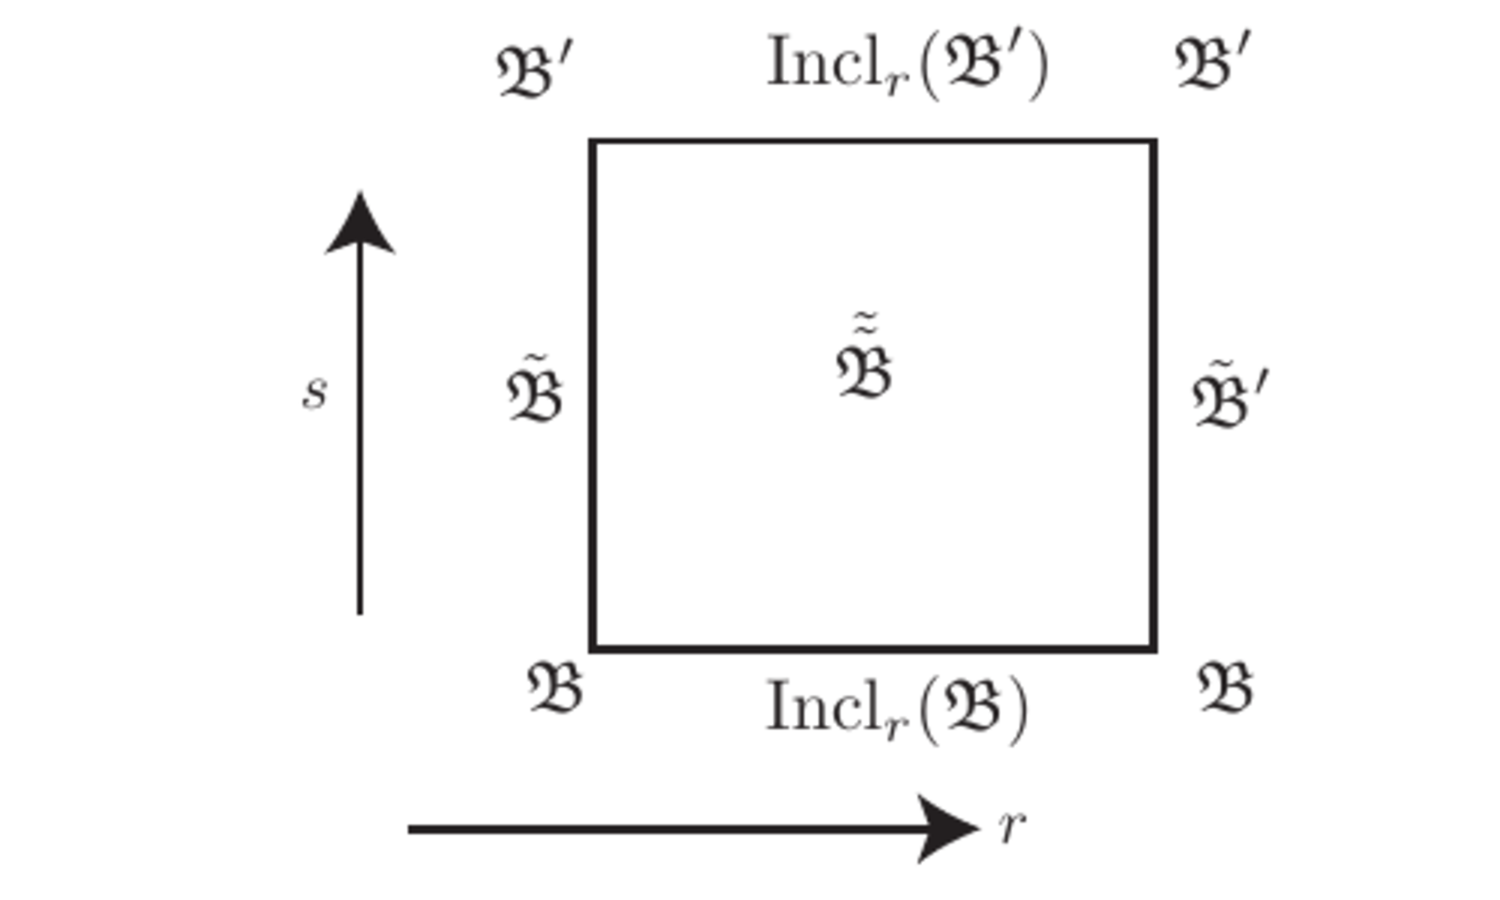
\includegraphics[width=.48\textwidth]{chapters/ch07-transversality/figures/phys-639-figure-7-4-15-math-final-crop.png}
\par\smallskip
{\renewcommand{\thefigure}{7.4.15}\refstepcounter{figure}
\normalfont\bfseries 图~\thefigure\label{fig:7-4-15}}
\end{minipage}\par\medskip

\begin{proof}
仿照式~\eqref{eq:7-4-133}，得到有隙滤过
微分分次李代数同态
\[
\widetilde\Phi\colon
\operatorname{Poly}
\bigl([0,1]_r\times[0,1]_s,
\operatorname{Der}B(C[1])\bigr)
\longrightarrow
\operatorname{Der}B
\bigl(
\operatorname{Poly}([0,1]_r\times[0,1]_s,C)[1]
\bigr).
\]
其余证明与定理~\ref{thm:7-4-132} 的证明类似。
\end{proof}

\begin{remark}{7.4.136}\label{rem:7-4-136}
在第 3.6、4.3 节中，
我们为滤过 $A_\infty$ 代数
$(C,\mathfrak m)$ 配置了 $\mathcal M(C)$。
它与本小节讨论的
$\mathcal M(\operatorname{Der}B(C[1]))$
有如下关系。
考虑 $(C,\mathfrak m)$ 的对称化
$(C,\mathfrak l)$（见定义 A3.7）。
容易看出
\[
\mathcal M(C,\mathfrak m)
=\mathcal M(C,\mathfrak l).
\]

另一方面，定义伴随滤过 $L_\infty$ 同态
\[
\operatorname{ad}\colon
(C,\mathfrak l)
\longrightarrow
\operatorname{Der}B(C[1])
\]
如下：
\begin{equation}
\begin{aligned}
&\operatorname{ad}(y_1,\ldots,y_k)(\mathbf x)\\
&\quad=
\frac{1}{k!}
\sum_{\sigma\in\mathfrak S_k}\sum_c
(-1)^{*(\sigma,c)}
\mathbf x_c^{(k+1;1)}
\otimes y_{\sigma(1)}
\otimes\mathbf x_c^{(k+1;2)}\\
&\qquad\qquad\otimes\cdots\otimes
\mathbf x_c^{(k+1;k)}
\otimes y_{\sigma(k)}
\otimes\mathbf x_c^{(k+1;k+1)}.
\end{aligned}
\tag{7.4.137}\label{eq:7-4-137}
\end{equation}
这里
\[
\Delta^k\mathbf x
=\sum_c
\mathbf x_c^{(k+1;1)}\otimes\cdots\otimes
\mathbf x_c^{(k+1;k+1)}
\]
（见约定 (Conv.3) 中的式 (1.1.35)），并且
\[
\begin{aligned}
*(\sigma,c)
={}&
\sum_{\substack{i<j\\\sigma(i)>\sigma(j)}}
\deg' y_i\deg' y_j\\
&+
\sum_{i<j}
\deg'\mathbf x_c^{(k+1;j)}
\deg' y_{\sigma(i)}.
\end{aligned}
\]
容易证明，伴随同态是严格滤过 $L_\infty$ 同态。
注意，当 $C$ 是结合代数时，
伴随同态对应于从 $C$ 取交换子所得李代数的伴随表示。

伴随同态诱导映射
\[
\operatorname{ad}_*\colon
\mathcal M(C,\mathfrak l)
\longrightarrow
\mathcal M\bigl(\operatorname{Der}B(C[1])\bigr).
\]
对
$b\in\widehat{\mathcal M}(C,\mathfrak m)$
及 $\mathfrak B=\operatorname{ad}_*(b)$，有恒等式
\[
\mathfrak m_k^b(x_1,\ldots,x_k)
=\mathfrak m(e^bx_1e^b\cdots e^bx_ke^b)
=\mathfrak m_k^{\mathfrak B}(x_1,\ldots,x_k).
\]
\end{remark}
